\section{Results and discussion}
\subsection{How many states, and is training stable?}
\begin{figure}[t]
\centering
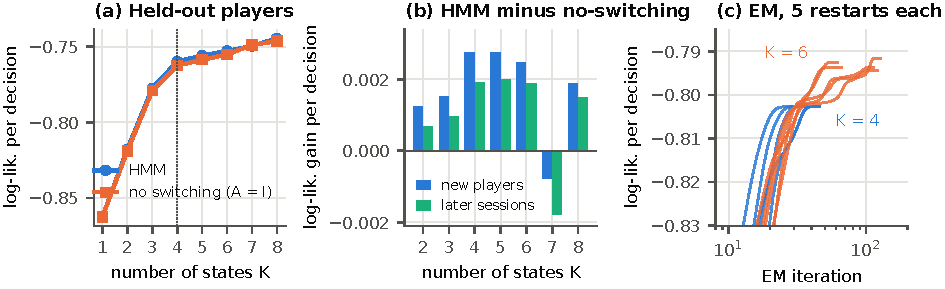
\includegraphics[width=\linewidth]{../figures/fig_selection.pdf}
\caption{(a) Held-out log-likelihood per decision against the number of states, for the HMM and for the same model with no switching. (b) Their difference. (c) Training log-likelihood during EM for five random starts each.}
\label{fig:selection}
\end{figure}
We swept $K=1,\dots,8$ (the proposal's 3 to 5, extended to see the shape). There is a clear elbow at $K=4$ (Figure~\ref{fig:selection}a; Table~\ref{tab:ll} in the appendix): on new players the log-likelihood per decision is $-0.8625$ with no hidden state, $-0.7776$ with three states, $-0.7598$ with four and $-0.7559$ with five. Held-out likelihood and BIC keep creeping up to $K=8$ (1.9 million decisions can always support a finer partition of players), so we choose $K$ by the elbow and by stability.

\textbf{Convergence.} The objective never decreased in any run. At $K=4$ all five starts reach the same optimum (to five decimals) in 32 to 46 iterations. From $K=5$ the starts end in different local optima (spread 0.003, Figure~\ref{fig:selection}c) after long plateaus, and at $K=7$ the best HMM found is worse on held-out data than the no-switching model nested inside it. Five restarts suffice at $K=4$ and not beyond.

\textbf{The uncomfortable baseline.} The no-switching model, in which a session keeps one mode throughout, reaches $-0.7626$ against the HMM's $-0.7598$. Hidden states are worth 0.103 nats per decision over $K=1$; letting the state \emph{change} within a session is worth 0.003 (Figure~\ref{fig:selection}b). Almost all the HMM learns is \emph{which kind of player this is}.

\textbf{Scalability.} Cost is linear in hands and quadratic in $K$; the whole sweep (76 fits) takes about ten minutes on 12 cores. With 295 parameters for 1.9M decisions, more data of the same kind would not change the pooled model.

\subsection{What the four states are}
\begin{figure}[t]
\centering
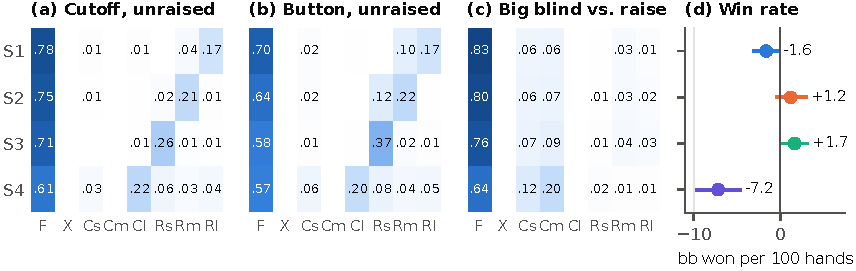
\includegraphics[width=\linewidth]{../figures/fig_states.pdf}
\caption{(a--c) Learned emission probabilities of the four states in three of the ten contexts. F fold, X check, C call and R raise at a small, medium or large size. (d) Win rate of held-out players grouped by the state they occupy most, with 95\% bootstrap intervals.}
\label{fig:states}
\end{figure}
\begin{table}[t]
\caption{The four states. Left: implied by the emission matrix (VPIP: share of hands in which money is put in voluntarily; PFR: share raised pre-flop; limp: share of unraised pots entered by calling; dwell: expected hands in the state). Right: held-out players grouped by the state they occupy most; \$0.25 is the share of their hands at the lowest stake; aggression (post-flop bets and raises per call) and win rate are never seen by the model.}
\label{tab:states}
\centering\small
\setlength{\tabcolsep}{2.6pt}
\begin{tabular}{lrrrlr|rrrr}
\toprule
 & \multicolumn{5}{c|}{Implied by emissions} & \multicolumn{4}{c}{Held-out players}\\
State (style, raise size) & VPIP & PFR & Limp & Usual raise & Dwell & Players & \$0.25 & Aggr. & Win rate, bb/100\\
\midrule
S1 tight, big & 19\% & 14\% & 3\% & large (79\%) & 1063 & 501 & 89\% & 2.6 & $-1.6$ $[-3.0,-0.3]$\\
S2 aggressive, pot-size & 23\% & 17\% & 3\% & medium (74\%) & 654 & 159 & 18\% & 2.6 & $+1.2$ $[-0.4,+2.9]$\\
S3 aggressive, small & 26\% & 20\% & 2\% & small (80\%) & 738 & 290 & 2\% & 2.7 & $+1.7$ $[+0.3,+3.1]$\\
S4 loose-passive & 37\% & 9\% & 29\% & mixed & 381 & 359 & 59\% & 1.9 & $-7.2$ $[-9.7,-4.7]$\\
\bottomrule
\end{tabular}
\end{table}
\textbf{The states match known style categories} (Figure~\ref{fig:states}, Table~\ref{tab:states}). S4 is the textbook loose-passive player: it enters 37\% of pots but raises 9\%, and limps 29\% of the time where the others limp 2 to 3\%. S1 to S3 are aggressive styles that raise nearly every pot they enter.

\textbf{They predict what the model never saw.} Held-out players who live mostly in S4 lose 7.2\bb\ per 100 hands (95\% interval $-9.7$ to $-4.7$), are the least aggressive after the flop and play the fewest hands: the recreational ``calling station''. S3 is the only group that wins after the rake.

\textbf{An unintended discovery.} S1, S2 and S3 differ mostly in the \emph{size} of their raises, and raise size is largely a convention of the game being played: 89\% of the hands of S1 players are at the \$0.25 stake and 98\% of those of S3 players at the higher stakes. The model was never told the stake and rediscovered it. A correct inference, and a warning that a fine alphabet lets states latch on to stable conventions.

\textbf{The states are traits.} Expected time in a state, $1/(1-A_{ii})$, is 381 to 1{,}063 hands, longer than the median session. On held-out players the Viterbi path changes state 0.44 times per 1{,}000 hands, 88\% of sessions have no change, and the average player spends 89\% of their hands in one state. The answer to question 1 is yes, with the qualification that the modes are styles of players, not moods.
